\documentclass[tikz,border=5pt]{standalone}
\usepackage{tikz}
\usetikzlibrary{arrows.meta}

\begin{document}

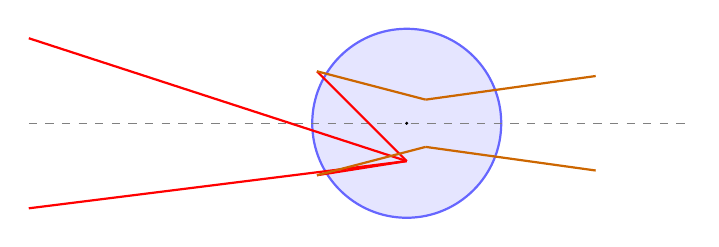
\begin{tikzpicture}[scale=1.2,
    ray/.style={red, thick},
    refracted/.style={orange!80!black, thick},
    sphere/.style={draw=blue!60, fill=blue!10, thick}
]

% Sphere (trapped particle)
\draw[sphere] (0,0) circle (1);
\draw[circle, fill=black!100] (0,0) circle (0.01);

% Beam axis
\draw[dashed, gray] (-4,0) -- (3,0);

% Focus point (left of sphere center)
\coordinate (F) at (0,-0.4);

% Incoming rays converging toward focus
\draw[ray] (-4,0.9) -- (F);
% \draw[ray] (-4,0.45) -- (F);
% \draw[ray] (-4,-0.45) -- (F);
\draw[ray] (-4,-0.9) -- (F);

% Continue rays to sphere surface
\draw[ray] (F) -- (-0.95,0.55);
% \draw[ray] (F) -- (-0.95,0.25);
% \draw[ray] (F) -- (-0.95,-0.25);
\draw[ray] (F) -- (-0.95,-0.55);

% Refracted rays inside sphere
\draw[refracted] (-0.95,0.55) -- (0.2,0.25);
% \draw[refracted] (-0.95,0.25) -- (0.4,0.1);
% \draw[refracted] (-0.95,-0.25) -- (0.4,-0.1);
\draw[refracted] (-0.95,-0.55) -- (0.2,-0.25);

% Exiting rays
\draw[refracted] (0.2,0.25) -- (2,0.5);
% \draw[refracted] (0.4,0.1) -- (2,0.2);
% \draw[refracted] (0.4,-0.1) -- (2,-0.2);
\draw[refracted] (0.2,-0.25) -- (2,-0.5);

% Labels
% \node at (0,-1.5) {Dielectric sphere};
% \node[red] at (-2.2,1.3) {Focused laser rays};

\end{tikzpicture}

\end{document}